\section{Algebraische Strukturen und Matrizen}

\begin{definition}[Gruppe]
	Sei $G$ eine Menge. $\langle G, \cdot, 1 \rangle$ ist eine \emph{Gruppe}, falls gilt:
	\begin{enumerate}[noitemsep]
		\item Abgeschlossenheit: $\cdot : G \times G \rightarrow G$
		\item Assoziativität: $\forall a,b,c \in G : a \cdot (b \cdot c) = (a \cdot b) \cdot c$
		\item Neutrales Element: $\forallin{a}{G}: a \cdot 1 = a = 1 \cdot a$
		\item Inverses Element: $\forallin{a}{G}: \exists a^{-1} \in G: a \cdot a^{-1} = 1 = a^{-1} \cdot a$
	\end{enumerate}

	Die Gruppe heißt endlich, falls gilt: $|G| < \infty$. $G$ heißt \emph{kommutativ}, falls zusätzlich gilt:
	\begin{description}
		\item $\forallin{a,b}{G}: a \cdot b = b \cdot a$
	\end{description}
\end{definition}

\begin{definition}[Körper]
	Eine Menge $\fieldk$ mit zwei Verknüpfungen, geschrieben $+$ und $\cdot$, $\langle \fieldk,+,\cdot \rangle$, heißt \emph{Körper} wenn folgendes gilt:
	
	\begin{enumerate}[noitemsep]
		\item $\langle \fieldk, +, 0 \rangle$ ist eine kommutative Gruppe
		\item $\langle \fieldk, \cdot, 1 \rangle$ ist eine kommutative Gruppe
		\item Distributivität: $\forallin{a,b,c}{\fieldk}: a \cdot b + a \cdot c = a \cdot (b +c)$
	\end{enumerate}
\end{definition}

\begin{definition}[Matrix]
	Sei $\fieldk$ ein beliebiger Körper und $m,n \in \naturalset \setminus \{0\}$. Eine Abbildung $\setonetom \times \setoneton \rightarrow \fieldk$ heißt \emph{Matrix}. Man schreibt:

	\begin{align*}
		\begin{pmatrix}
			a_{1,1} & \dots & a_{1,n} \\
			\vdots  &       &         \\
			a_{m,1} & \dots & a_{m,n}
		\end{pmatrix}
		= (\subij{a})_{1 \leq i \leq m \atop 1 \leq j \leq n}
		= (\subij{a}) = A \in \fieldk^{\mtimesn}
	\end{align*}	

	Eine $1 \times n$ Matrix heißt \emph{Zeilenvektor}, eine $m \times 1$ Matrix heißt \emph{Spaltenvektor}. Man schreibt mit $\fieldk^m = \fieldk^{m \times 1}$ und nennt dies $m$-dimensionaler Standardraum. 
\end{definition}

\begin{definition}[Eigenschaften von Matrizen]
	Es gilt:
	\begin{enumerate}[noitemsep]
		\item Zwei Matrizen $A,B$ sind gleich, wenn beide $\mtimesn$ Matrizen sind und $\forallin{i}{\setonetom}, \forallin{j}{\setoneton} : \subij{a} = \subij{b}$.
		\item Eine $\mtimesn$ Matrix heißt \emph{quadratisch}, falls $m=n$
		\item Für $A = (\subij{a}) \in \fieldkmtimesn$ ist $A^T = (a_{j,i}) \in \fieldk^{n \times m} $ die \emph{transponierte Matrix}
		\item Eine Matrix heißt \emph{symmetrisch}, wenn $A^T = A$ gilt.
		\item 	Elemente aus $\fieldk$ heißen auch \emph{Skalare}. 
	\end{enumerate}

\end{definition}

\begin{definition}[Rechnen mit Matrizen]
	Für $A, B \in \fieldkmtimesn, D \in \fieldk^{n \times l}, s \in \fieldk$ gilt:
	\begin{description}[noitemsep]
		\item $A + B := (\subij{a} + \subij{b}) \in \fieldkmtimesn$
		\item $s \cdot A = (s \cdot \subij{a}) \in \fieldkmtimesn$
		\item $A \cdot D = C = (\subij{c}) \in \fieldk^{m \times l}$ mit $\subij{c} = \sum_{k=1}^{n}a_{i,k} d_{k,j}$
	\end{description}
\end{definition}

\pagebreak

\begin{satz}[Rechenregeln mit Matrizen]
	Für Matrizen $A,B,C$ und Skalare $s,t$ mit definierten Summen und Matrizen gilt:
	\begin{multicols}{2}
		\begin{enumerate}[noitemsep]
			\item $s \cdot (A + B) = s \cdot A + s \cdot B$
			\item $(s+t) \cdot A = s \cdot A + t \cdot A$
			\item $s \cdot (t \cdot A) = (s \cdot t) \cdot A$
			\item $1 \cdot A = A$
			\item $(A \cdot B) \cdot C = A \cdot (B \cdot C)$
			\item $A \cdot (B + C) = A \cdot B + A \cdot C$
			\item $(A + B) \cdot C = A \cdot C + B \cdot C$
			\item $I_n \cdot A = A = A \cdot I_n$ wobei \\
			  $I_n = \begin{pmatrix}
			  1 &        & 0 \\
			    & \ddots &   \\
			  0 &        & 1
			\end{pmatrix}$ Einheitsmatrix
		\end{enumerate}
	\end{multicols}
\end{satz}


\section{LGS}

\begin{definition}[Lineares Gleichungssystem]
	Eine Gleichung der Form $Ax=b$ mit $A \in \fieldkmtimesn, b \in \fieldk^m$ heißt lineares Gleichungssystem (LGS). Die Lösungsmenge ist die Menge aller $x \in \fieldk^n$ sodass $Ax = b$ gilt. $A$ heißt \emph{Koeffizientenmatrix}. Wird $b$ an $A$ angeheftet, schreibt man $(A|b) \in \fieldk^{m \times (n+1)}$ und nennt dies \emph{erweiterte Koeffizientenmatrix}.
\end{definition}

\begin{definition}[homogenes LGS]
	Gilt $b = 0$, so heißt das LGS \emph{homogen}, ansonsten nennt man es \emph{inhomogen}.
\end{definition}

\begin{satz}[Zeilenoperationen]
	Elementare Zeilenoperationen vereinfachen das LGS ohne die Lösungsmenge zu verändern:
	\begin{description}[noitemsep]
		\item Typ I: Vertauschen zweier Zeilen
		\item Typ II: Multiplizieren einer Zeile mit einem Skalar $s \in \fieldk \setminus \{0\}$
		\item Typ III: Addieren des s-fachen einer Zeile zu einer anderen
	\end{description}
\end{satz}

\begin{definition}[Zeilenstufenform]
	$A$ ist in Zeilenstufenform, wenn gilt:
	\begin{enumerate}[noitemsep]
		\item beginnt eine Zeile mit $k$ Nullen, so stehen unter diesen Nullen lauter Nullen
		\item unter dem ersten Eintrag $\neq 0$ einer jeden Zeile stehen lauter Nullen
		\item $A$ ist in strenger Zeilenstufenform wenn zusätzlich gilt: über dem ersten Eintrag $\neq 0$ einer jeden Zeile stehen lauter Nullen
	\end{enumerate}
\end{definition}

\begin{satz}
	Möglichkeiten der Lösungsmenge eines LGS:
	\begin{description}[noitemsep]
		\item Unlösbar $\leftrightarrow$ der erste Eintrag $\neq 0$ einer Zeile ist an Spalte $n+1$
		\item Eindeutig lösbar $\leftrightarrow$ Anzahl der Zeilen $\neq 0$ ist gleich Anzahl der Spalten und der erste Eintrag $\neq 0$ einer jeden Zeile ist an Spalte $n$.
		\item Uneindeutig lösbar $\leftrightarrow$ Anzahl der Zeilen $\neq 0$ ist kleiner der Anzahl der Spalten und der erste Eintrag $\neq 0$ einer jeden Zeile ist nicht an Spalte $n+1$.		
	\end{description}
\end{satz}

\begin{definition}[Rang einer Matrix]
	Sei $A'$ eine Matrix in Zeilenstufenform, die aus $A$ durch elementare Zeilenoperationen hervorgegangen ist. $rng(A)$ ist dann die Anzahl der Zeilen von $A'$ die mindestens einen Eintrag $\neq 0$ haben.
\end{definition}

\pagebreak

\section{Vektorräume}

\begin{definition}[Vektorraum]
	Sei $\langle \fieldk, +, \cdot \rangle $ ein Körper. Ein \emph{Vektorraum} über $\fieldk$ ist eine Menge $V$ zusammen mit zwei Abbildungen:
	
	\begin{description}[noitemsep]
		\item $\oplus : V \times V \rightarrow V : (v,w) \mapsto v \oplus w$
		\item $\odot  : \fieldk \times V \rightarrow V : (a, w) \mapsto a \odot w$
	\end{description}
	sodass gelte:
	\begin{enumerate}[noitemsep]
		\item $\langle V, \oplus, 0 \rangle$ bilden eine kommutative Gruppe
		\item $\forallin{a}{\fieldk}, \forallin{w,v}{V}: a \odot (v \oplus w) = (a \odot v) \oplus (a \odot w)$
		\item $\forallin{a,b}{\fieldk}, \forallin{v}{V}: (a + b) \odot v = (a \odot v) \oplus (a \odot v)$
		\item $\forallin{a,b}{\fieldk}, \forallin{v}{V}: (a \cdot b) \odot v = (a \odot b) \odot v$
		\item $\forallin{v}{V} : 1 \odot V = V$	
	\end{enumerate}
	Elemente aus $V$ heißen Vektoren, Elemnte aus $\fieldk$ Skalare. $\odot, \oplus, \boldsymbol{0}$ als Unterscheidung der Addition, Multiplikation in $\fieldk$ und $\boldsymbol{0}$ als Unterscheidung zur skalaren Null.
\end{definition}

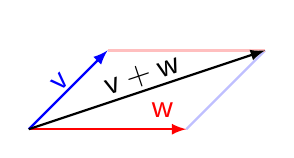
\begin{tikzpicture}\large
% Punkte
\coordinate (A) at (0,0) {};
\coordinate (B) at (2,0) {};
\coordinate (C) at (1,1) {};
\coordinate (D) at (3,1) {};

% Draw the triangle
\draw[thick, blue!25]  (B) -- (D) node[sloped,midway,above] {};
\draw[thick, red!25]   (C) -- (D) node[sloped,midway,above] {};
\draw[->, thick, red,   arrows={-latex}]  (A) -- (B) node[sloped,right=-0.3cm, above] {$\mathsf{w}$};
\draw[->, thick, blue,  arrows={-latex}]  (A) -- (C) node[sloped,midway,above=-0.1cm] {$\mathsf{v}$};
\draw[->, thick, black, arrows={-latex}]  (A) -- (D) node[sloped,midway,above=-0.1cm] {$\mathsf{v+w}$};
\end{tikzpicture}
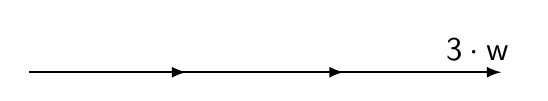
\begin{tikzpicture}\large
% Punkte
\coordinate (A) at (0,0) {};
\coordinate (B) at (6,0) {};
% Draw the triangle
\draw[->, thick, black,   arrows={-latex}]  (A) -- (2,0) node[sloped,right=-0.3cm, above] {};
\draw[->, thick, black,   arrows={-latex}]  (A) -- (4,0) node[sloped,right=-0.3cm, above] {};
\draw[->, thick, black,   arrows={-latex}]  (A) -- (B) node[sloped,right=-0.3cm, above] {$\mathsf{3 \cdot w}$};
\end{tikzpicture}

\begin{satz}[Rechenregeln im Vektorraum]
	Es gilt für $a \in \fieldk, v \in V:$
	\begin{enumerate}[noitemsep]
		\item $a \cdot \boldsymbol{0} = \boldsymbol{0} = 0 \cdot v$
		\item $(-a) \cdot v = a \cdot (-v) = - (a \cdot v)$
		\item $a \cdot v = \boldsymbol{0} \rightarrow (a = 0) \lor (v = \boldsymbol{0})$
	\end{enumerate}
\end{satz}

\begin{definition}[Untervektorraum]
	Sei $V$über $\fieldk$ ein Vektorraum. $U \subseteq V$ heißt \emph{Untervektorraum}, falls gilt:
	\begin{enumerate}[noitemsep]
		\item $U \neq \emptyset$
		\item $\forallin{v,w}{U} : (v+w) \in U$
		\item $a \in \fieldk, v \in U \rightarrow (a \cdot v) \in U$
	\end{enumerate}
	Darauß folgt:
	\begin{enumerate}[noitemsep]
		\item $\langle U, + \rangle$ ist eine Untergruppe von $\langle V, + \rangle$
		\item $U$ enthält automatisch den Nullvektor
		\item $U$ ist selbst wieder ein $\fieldk$ Vektorraum bzgl. $+$ und $\cdot$
	\end{enumerate}
\end{definition}

\begin{satz} Seien $U_1, U_2 \subseteq V$ Untervektorräume. Dann gilt:
	\begin{enumerate}[noitemsep]
		\item $U_1 \cap U_2 \subseteq V$ ist ein Unterraum
		\item $U_1 + U_2 := \{v + w | v \in U_1, w \in U_2\} \subseteq V$ ist ein Unterraum
		\item $Ist M \neq \emptyset$ eine Menge deren Elemente selbst Unterräume sind, dann ist auch $\bigcap_{u \in M} u \in V$ ein Unterraum
	\end{enumerate}
\end{satz}

\pagebreak

\begin{definition}[Erzeugter Unterraum]
	Sei $S \subseteq V, M := \{U \subseteq V \medspace \lvert \medspace U$  ist ein Unterraum und $S \subseteq U \}. \langle S \rangle := \bigcap_{u \in M} u \subseteq V $ und $\langle S \rangle$ heißt der von $S$ erzeugte bzw. aufgespannte Unterraum. 
	
	Falls $S = \{v_1,\dots, v_n\}$ schreibt man auch $\langle S \rangle = \langle v_1, \dots, v_n \rangle$. Per Konstruktion ist $\langle S \rangle$ der kleinste Unterraum, der $S$ als Teilmenge enthält. Jeder Unterraum von $V$, der $S$ als Teilmenge enthält, enthält $\langle S \rangle$.
\end{definition}

\section{Linearkombinationen}
\begin{definition}[Linearkombination]
	Sei $\fieldk$ ein Körper, $V$ ein $\fieldk$-Vektorraum.
	\begin{enumerate}[noitemsep]
		\item Eine Linearkombination von $\suboneton{v} \in V$ ist eine Summe der Form $\sum_{k}^{n}a_kv_k$ für $\suboneton{a} \in \fieldk$
		\item Sei $S \subseteq V$. Ein Vektor $v \in V$ heißt Linearkombination von $S$, falls es ein $n \in \naturalset$ und $\suboneton{v} \in S$ gibt, sodass $v$ eine Linearkobination von $\suboneton{v}$ ist, d.h. $v = \sum_{k=1}^{n} a_kv_k$. Gilt $S = \emptyset$,  ist der Nullvektor die einzige Linearkombination
	\end{enumerate}
\end{definition}

\begin{definition}
	Sei $V$ ein $\fieldk$-Vektorrau, $S \subseteq V$. $\langle S \rangle = \{v \in V | v$ ist Linearkombination von $ S \}$. Insbesondere gilt: $\suboneton{v} \in V \rightarrow \langle \suboneton{v} \rangle = \{a_1v_1, \dots, a_nv_n | \ a_i \in \fieldk\}$
\end{definition}

\begin{definition}[Lineare Unabhängigkeit]
	Vektoren $\suboneton{v}$ heißen
	\begin{enumerate}[noitemsep]
		\item \emph{linear unabhängig}, wenn: $a_1v_1 + \dots + a_nv_n = 0 \rightarrow a_1,\dots, a_n = 0$ mit $a_i \in \fieldk$, d.h. die einzige Möglichkeit, aus $\suboneton{v}$ den Nullvektor linear zu kombinieren, ist $0v_1 + \dots + 0v_n$
		\item \emph{linear abhängig}, wenn sie nicht linear unabhängig sind. Eine Teilmenge $S \subseteq V$ heißt \emph{linear unabhängig}, wenn $\forallin{n}{\naturalset}$ und $\suboneton{v} \in S$ gilt: $\suboneton{v}$ sind linear unabhängig.
	\end{enumerate}
Per Definition ist $S = \emptyset$ linear unabhängig. Enthält $S$ den Nullvektor oder $\{\suboneton{v}\}$ sodass $v_i = 0$ für ein $i$, dann ist $S$ bzw. $\{ \suboneton{v} \}$ ist linear unabhängig.
\end{definition}

\begin{satz}[Rang einer Matrix]
	Seien $\suboneton{v} \in \fieldk$ Vektoren. Bilde die Matrix $A = (v_a|\dots|v_n) \in \fieldkmtimesn$ wobei $v_i$ Spalten von $A$ sind. $\{\suboneton{v}\}$ sind linear unabhängig $\leftrightarrow rang(A) = n$. Es gilt $rang(A) \leq min\{m,n\}$. 
	
	Gelte nun $n < m$, so folgt $rang(A) \leq m < n$, d.h. also Vektoren im $\fieldk^n$ mit $m > n$ sind automatisch linear abhängig.
\end{satz}
\pagebreak

\section{Basen}
\begin{definition}[Basis]
	 Sei $V$ ein Vektorraum über $\fieldk$. Sei $S \subseteq V$.
	\begin{enumerate}[noitemsep]
		\item $S$ heißt Erzeugendensystem, wenn $\langle S \rangle = V$
		\item $S$ heißt Basis von $V$, wenn $S$ Erzeugendensystem und linear unabhängig ist
	\end{enumerate}
	D.h. $S$ ist Basis von $V$ gdw jeder Vektor von $V$ lässt sich in eindeutigerweise als Linearkombination von Vektoren aus $S$ schreiben
\end{definition}

\begin{satz}
	$S$ ist eine Basis von $V$
	\begin{enumerate}[noitemsep]
		\item $\leftrightarrow S$ ist eine maximimal linear unabhängige Teilmenge, d.h.
		\begin{description}[noitemsep]
			\item $S$ ist linear unabhängig
			\item $\forallin{v}{V}, v \notin S : S \cup \{v\}$ ist linear abhängig
		\end{description}
		\item $\leftrightarrow S$ ist minimales Erzeugendensystem, d.h.
		\begin{description}[noitemsep]
			\item $S$ ist Erzeugendensystem
			\item $\forallin{v}{S}$ ist $S \setminus \{v\}$ kein Erzeugendensystem
		\end{description}
	\end{enumerate}
	Folgerungen:
	\begin{description}[noitemsep]
		\item Wenn $V$ ein endliches Erzeugendensystem besitzt, dann besitzt $V$ eine Basis.
		\item Sei $V$ ein $\fieldk$ - Vektorraum. Dann besitzt $V$ eine Basis
		\item Sei $V$ ein $\fieldk$ - Vektorraum. Sei $E$ ein endliches Erzeugendensystem und $U \subseteq V$ linear unabhängig. Dann gilt $|U| \leq |E|$ 
		\item Sei $V$ ein $\fieldk$ - Vektorraum mit endlichem Erzeugendensystem. Dann sind alle Basen von $V$ endlich und besitzen gleich viele Elemente
	\end{description}
\end{satz}

\begin{definition}[Dimension]
	Die Anzahl der Elemente einer Basis von $V$ heißt \emph{Dimension}, $\dim(V)$.
	
	Folgerungen:
	\begin{satz}
		Sei $A \in \fieldkmtimesn, L := \{x \in \fieldk^n | Ax = 0 \}$. Dann gilt: $dim(L) = n-rang(A)$. 
		Sei $A = \langle \suboneton{v} \rangle \subseteq \fieldk^n$. Stelle $A \in \fieldkmtimesn$ auf, die die $V_i$ als Zeilen enthält. Bringe $A$ mittels Gauß in Zeilenstufenform. Die Zeilen $\neq 0$ bilden eine Basis von $V$. 
	\end{satz}
\end{definition}

\begin{satz}
	Sei $V$ ein $\fieldk$-Vektorraum, $\suboneton{v}$ paarweise verschieden, $S = \{\suboneton{v}\}$.
	\begin{enumerate}[noitemsep]
		\item $S$ ist eine Basis von $V \leftrightarrow dim(V) = n$ und $S$ linear unabhängig.
		\item $n < dim(V) \rightarrow V \neq \langle S \rangle$
		\item $n > dim(V) \rightarrow S$ ist linear unabhängig 
	\end{enumerate}
\end{satz}

\begin{satz}[Basisergänzungssatz]
	Sei $V$ ein endlich dimensionaler $\fieldk$ Vektorraum, $S \subseteq V$ linear unabhängig. Dann gibt es eine Basis $B$ von $V$ und $S \subseteq B$.
\end{satz}

\begin{satz}
	Sei $V$ ein $\fieldk$ - Vektorraum, $U \subseteq V$ Unterraum von $V$.
	\begin{enumerate}[noitemsep]
		\item $dim(U) \leq dim(V)$
		\item $dim (U) = dim(V) < \infty \rightarrow U = V$
	\end{enumerate}
\end{satz}

\section{Lineare Abbildungen}

\begin{definition}[Lineare Abbildung]
	Seien $V, W$ Vektorräume über $\fieldk$. $\function{\phi}{V}{W}$ heißt \emph{Lineare Abbildung}, falls
	\begin{enumerate}[noitemsep]
		\item $\forallin{v, v'}{V}: \phi(v + v') = \phi(v) + \phi(v')$
		\item $\forallin{v}{V}: \forallin{a}{\fieldk}: \phi(a \cdot v) = a \cdot \phi(v)$
	\end{enumerate}
\end{definition}

\begin{definition}
	Homomorphismus $Hom := \{\phi : V \rightarrow W \medspace | \medspace \phi \medspace \textnormal{ist lineare Abbildung}\}$.  $Hom(V,W)$ ist ein Vektorraum mit
	\begin{description}[noitemsep]
		\item $+ : \phi + \psi : V \rightarrow W : \phi(v) + \phi(w) = \phi(v + w) \in Hom(V,W)$
		\item $\cdot : \lambda \cdot \phi : V \rightarrow W : v \mapsto \lambda \phi(v) = \phi(\lambda v) \in Hom(V,W)$
	\end{description}

	Gilt $V = W$, so ist $Hom(V,V) := End(V)$ Endomorphismus. Seien $\phi, \psi \in End(V)$. Dann gilt:: $\phi \circ \psi : V \rightarrow V : v \mapsto \phi(\psi(v)) \in End(V)$
\end{definition}

\begin{definition}
	$Kern(\phi) := \{v \in V \medspace | \medspace \phi(v) = 0\}$, $Bild(\phi) := \{\phi(v) \medspace | \medspace v \in V\}$. 
		Es gilt:	

	\begin{enumerate}[noitemsep]
		\item $Kern(\phi) \subseteq V$ ist ein Unterraum von V
		\item $Bild(\phi) \subseteq W$ ist ein Unterraum von W
		\item $\phi$ ist injektiv $\leftrightarrow Kern(\phi) = \{0\}$
	\end{enumerate}
\end{definition}

\begin{definition}[Isomorphismus]
	$\phi$ heißt \emph{Isomorphismus}, falls $\phi$ bijektiv ist. Zwei Vektorräume $V,W$ heißen \emph{isomorph}, falls es einen Isomorphismus $\phi : V \rightarrow W$ gibt.
\end{definition}

\begin{satz}[Dimensionssatz]
	Seien $V,W$ Vektorräume, $\function{\phi}{V}{W}$ lineare Abbildung. Es gilt: $dim(V) = dim(Kern(\phi)) + dim(Bild(\phi))$
\end{satz}

\begin{definition}
	Lineare Abbildungen lassen sich als Matrizen $A \in \fieldkmtimesn$ darstellen: $\phi_A : \fieldk^n \rightarrow \fieldk^m : v \mapsto Av$ Darauß folgt:
	\begin{description}[noitemsep]
		\item $Kern(\phi_A) = \{v \in \fieldk^n \medspace | \medspace Av = 0\}$
		\item $dim(Kern(\phi_A)) = n - rang(A)$
		\item $dim(Bild(\phi_A)) = Rang(A)$
	\end{description}
\end{definition}

Für $\phi : V \rightarrow W$ linear, $dim(V) < \infty$, $dim(W) < \infty$ gilt: $\phi$ ist Isomorphismus $\leftrightarrow \phi$ ist injektiv $\leftrightarrow \phi$ ist surjektiv.

\begin{satz}
	Eine Matrix $A \in \fieldkntimesn$ ist invertierbar, wenn: $\exists B \in \fieldkntimesn : A \cdot B = I \rightarrow B = A^{-1}$.  A ist invertierbar $\leftrightarrow rang(A) = n$ und es gilt $A \cdot A^{-1} = A^{-1} \cdot A = I$ (links -und rechtsinvers).
\end{satz}

\begin{satz}
	Sei $V$ ein $\fieldk$ - Vektorraum, $B = \{\suboneton{v}\}$ eine Basis. Dann gilt:
	\begin{enumerate}[noitemsep]
		\item Eine lineare Abbildung $\phi : V \rightarrow W$ ist durch die Bilder der Basisvektoren eindeutig bestimmt, d.h. $\psi : V \rightarrow W$ lineare Abbildung und  $\forall i : \psi(v_i) = \phi(v_i) \rightarrow \psi = \phi $
		\item Seien $\suboneton{w}$ beliebige Elemente des Vektorraums $W$. Dann gibt es genau eine Abbildung $\phi : V \rightarrow W$ sodass $\forall i : \phi(v_i) = w_i$
	\end{enumerate} 
\end{satz}

\pagebreak

\section{Darstellungsmatrizen}

\begin{definition}[Darstellungsmatrix]
	Sei $\fieldk$ ein Körper, $V,W$ $\fieldk$ - Vektorräume mit Basis $B = \{\suboneton{v}\}, C = \{\suboneton{w}\}$. Sei $\function{\phi}{V}{W}$ eine lineare Abbildung.
	Dann gilt: $\forallin{j}{1, \dots , n}: \exists a_{i,j} \in \fieldk$ mit $\phi(v_j) = \sum_{i=1}^{m} a_{i,j} w_i$ (Koeffizienten der Linearkombination der Elemente aus $W$ entstehend aus $\phi$ linear kombiniert bzgl. $C$). 

	$A = \begin{pmatrix}
		a_{1,1} & \dots & a_{1,n} \\
		\vdots & & \\
		a_{m,1} & \dots & a_{m,n}
	\end{pmatrix} \in \fieldkmtimesn = (a_{i,j})$ heißt Darstellungsmatrix bzgl der Basen $B, C$. Man schreibt auch $D_{B,C}(\phi) = A \in \fieldkmtimesn$. Gilt $V=W, B=C$ auch einfach $D_B(\phi) \in \fieldk^{n \times n}$. Man kann aus $D_{B,C}(\phi)$ also alle $\phi(v_{i,j})$ eindeutig bestimmen und jede Matrix ist eine Darstellungsmatrix genau einer linearen Abbildung.
\end{definition}

\begin{definition}
	Sei $V = \fieldk^n, W=\fieldk^m$ mit den Standardbasen $B,C$ und $\function{\phi}{V}{W}$ lineare Abbildung. Sei $A=D_{B,C}(\phi)$. Dann ist $\phi = \phi_A : \fieldk^n \rightarrow \fieldk^m : v \mapsto Av$. Insbesondere sind alle Abbildungen von $v$ nach $W$ in der Form $\phi_A$ für ein $A \in \fieldkmtimesn$ und $A$ ist die Darstellungsmatrix von $\phi$ bzgl. der Standardbasen.
\end{definition}

\begin{satz}
	Seien $U,V,W \medspace \fieldk$ - Vektorräume, $\function{\phi}{U}{V}, \function{\psi}{V}{W}$ lineare Abbildungen. Seien $A,B,C$ Basen von $U,V,W$. Dann gilt: $D_{A,C}(\psi \circ \phi) = D_{B,C}(\psi) \cdot D_{A,B}(\phi)$
\end{satz}

\begin{satz}
	Seien $A \in \fieldk^{l \times m}, B \in \fieldkmtimesn, \function{\phi_A}{\fieldk^m}{\fieldk^l} : v \mapsto Av, \function{\phi_B}{\fieldk^n}{\fieldk^m} : w \mapsto Bw$. Dann gilt:  $\phi_A \circ \phi_B = \phi_{A \cdot B}$ und 
	 $\phi_{A^{-1}} = (\phi_A)^{-1}$
\end{satz}

\begin{satz}
	Sei $V$ ein $\fieldk$ - Vektorraum. $B = \{ \suboneton{v} \}, B'=\{\suboneton{v'}\}$ Basen. Dann gibt es eindeutige $a_{i,j} \in \fieldk$ sodass
	
	\begin{equation*}
		v_j' = \sum_{i=1}^{n} a_{i,j} \cdot v_{i,j}, \medspace S_{B,B'} := S = (a_{i,j}) \in \fieldkntimesn  
	\end{equation*}
	wird Basiswechselmatrix von $B$ nach $B'$ genannt. Umgekehrt gibt es eindeutige $b_{i,j} \in \fieldk$ sodass
	\begin{equation*}
		v_i  = \sum_{i=1}^{n} b_{i,j} \cdot v_i', \medspace S_{B',B} = T = (b_{i,j}) \in \fieldkntimesn 
	\end{equation*}
	heißt Basiswechselmatrix von $B'$ zu $B$. Dabei gilt: $S \cdot T = I_n$. $S$ ist also Inverse von $T$ und umgekehrt und $S_{B', B} = (S_{B,B'})^{-1}, S_{B,B'} = (S_{B',B})^{-1}$. Weiterhin gilt $D_{B'}(\phi) = S^{-1} \cdot D_B(\phi) \cdot S$
\end{satz}

\begin{definition}
	$GL_n(\fieldk) = \{A^{n \times n} \medspace | \medspace A \medspace \textnormal{ist invertierbar}\}$ heißt \emph{allgemein lineare Gruppe}. Zwei quadratische Matrizen $A,B \in \fieldkntimesn$ heißen ähnlich, wenn es ein $S \in GL_n(\fieldk)$ gibt sodass $B = S^{-1} \cdot A \cdot S$. Gibt es ein $T \in GL_n(\fieldk)$ sodass $B = T^{-1} \cdot A \cdot S$, so heißen $A,B$ äquivalent.
\end{definition}

\section{Determinanten} 

\begin{definition}[Symmetrische Gruppe]
	Sei $n \in \mathbb{Z}_{\geq 1}$. Die symmetrische Gruppe ist die Menge $S_n := \{ \sigma : \{ 1, \dots, n \} \rightarrow \{1, \dots, n\} \medspace | \medspace \sigma \medspace \textnormal{ist bijektiv}  \}$ mit $\langle S_n, \circ, Id \rangle$ und der Umkehrabbildung als Gruppenstruktur. Elemente aus $S_n$ heißen Permutationen. $S_n$ hat endliche viele Elemente mit $|S_n| = n!$
\end{definition}

\begin{definition}
	Sei $\sigma \in S_n$.
	\begin{enumerate}[noitemsep]
		\item $w(\sigma) := $ Anzahl der Paare $(i,j)$ mit $1 \leq i < j \leq n$ und $\sigma(i) > \sigma(j)$. Diese Paare heißen \emph{Fehlstellen}
		\item $sgn(\sigma) := (-1)^{w(\sigma)}$
	\end{enumerate}
\end{definition}

\begin{definition}[Permanente, Determinante]
	Sei $A = (a_{i,j}) \in \fieldkntimesn$ quadratische Matrix. Dann ist
	\begin{enumerate}[noitemsep]
		\item Die Permanente von $A$ ist $perm(A) = \sum_{\sigma \in S_n}(\Pi_{i=1}^n a_ {i, \sigma(i)})$
		\item Die Determinante von $A$ ist $det(A) = \sum_{\sigma \in S_n}(sgn(\sigma) \cdot \Pi_{i=1}^n a_ {i, \sigma(i)})$		
	\end{enumerate}
	Allgemein beschreibt die Determinante eine Funktion $A \mapsto det(A)$. Sie gibt an, wie sich das Volumen bei der durch die Matrix beschriebenen linearen Abbildung ändert.
\end{definition}

\begin{satz}
	Sei $A = (a_{i,j}) \in \fieldkntimesn$
	\begin{enumerate}[noitemsep]
		\item $det(A^T) = det(A)$
		\item Wenn in $A$ zwei Zeilen oder Spalten übereinstimmen, gilt $det(A) = 0$
	\end{enumerate}
\end{satz}

\begin{satz}[Determinantenmultiplikationssatz]
	Seien $A,B \in \fieldkntimesn$. Es gilt: $det(A \cdot B) = det(A) \cdot det(B)$. Folgerungen:
	
	\begin{enumerate}[noitemsep]
		\item $A$ ist regulär $\leftrightarrow det(A) \neq 0$. Ansonsten heißt $A$ singulär
		\item Sei $A$ regulär. Dann ist $det(A^{-1}) = \frac{1}{det(A)}$.
		\item Seien $A,B$ ähnlich. Dann gilt $det(A) = det(B)$ (Aus dieser Eigenschaft folgt die wohldefiniertheit der Determinante)
	\end{enumerate}
\end{satz}

\begin{satz}[Determinanten spezieller Matrizen] Es gilt:
	\begin{enumerate}[noitemsep]
		\item Diagonalmatrizen: $det( \left( \begin{smallmatrix}
		a_1 & & 0 \\
		& \ddots & \\
		0 & & a_n 
		\end{smallmatrix} \right) ) = a_1 \cdot \dots \cdot a_n$
		\item Obere (analog: untere) Dreiecksmatrizen: $det( \left( \begin{smallmatrix}
		a_1 & & * \\
		& \ddots & \\
		0 & & a_n 
		\end{smallmatrix}  \right) ) = a_1 \cdot \dots \cdot a_n$
		\item Matrizen in Block-Dreiecksgestalt: $A = \begin{pmatrix}
		B & 0 \\
		C & D 
		\end{pmatrix} \in \fieldkmtimesn$ mit $B \in \fieldk^{l \times l}, D \in \fieldk^{(n-l) \times (n-l)}, C \in \fieldk^{(n-l) \times l}$.
		Es gilt: $det(A) = det(B) \cdot det(D)$
	\end{enumerate}
\end{satz}


\section{Eigenwerte und Eigenvektoren}
\begin{definition}	
	Sei $A \in \fieldkntimesn; \lambda \in \fieldk $ heißt \emph{Eigenwert}, wenn es ein $v \neq 0 \in \fieldk^n$ gibt, sodass $Av = \lambda v$ gilt. $v$ heißt dann \emph{Eigenvektor} zum Eigenwert $\lambda$. Er ist ein Vektor, dessen Richtung durch $A$ (d.h. einer linearen Abbildung) nicht verändert wird. Lediglich seine Skalierung ändert sich.

	Der Eigenraum zum Eigenwert $\lambda$ ist definiert als $E_\lambda := \{x \in \fieldk^n \medspace | \medspace Ax = \lambda x \}$, d.h. die Menge aller Eigenvektoren zum Eigenwert $\lambda \cup \{0\}$. 
\end{definition}

\begin{definition}[Charakteristisches Polynom]
	Sei $A \in \fieldkntimesn$ quadratische Matrix. Dann heißt $\mathcal{X_A} = \mathcal{X}_A(x) := det(x \cdot I_n -A) \in \fieldk[X]$ \emph{charakteristisches Polynom} von $A$.
\end{definition}

\begin{satz}
	Die Eigenwerte einer quadratischen Matrix $A \in \fieldkntimesn$ sind gleich der Nullstellen des charakteristischen Polynoms von $A$. 
\end{satz}

\begin{definition}
	Ein Körper $\fieldk$ heißt algebraisch abgeschlossen, wenn jedes nicht-konstante Polynom $f \in \fieldk[X]$ in Linearfaktoren zerfällt. Beispiel: $\complexset$. Es folgt für $A \in \fieldkntimesn, n \geq 1$ und $\fieldk$ algebraisch abgeschlossen:
	\begin{description}[noitemsep]
		\item $A$ hat höchstens $n$ Eigenwerte und $A$ hat mindestens einen Eigenwert
	\end{description}
\end{definition}

\begin{definition}
	Sei $A \in \fieldkntimesn, \lambda \in \fieldk$ Eigenwert von $A$.
	\begin{enumerate}[noitemsep]
		\item Die algebraische Vielfachheit von $\lambda, m_a(\lambda),$ ist die Vielfachheit von $\lambda$ als Nullstelle von $\mathcal{X_A}$.
		\item Die geometrische Vielfachheit von $\lambda, m_g(\lambda,)$ ist die Dimension des zugehörigen EIgenraums.
	\end{enumerate}
\end{definition}

\begin{satz}
	Sei $A \in \fieldkntimesn, \lambda \in \fieldk$ Eigenwert von $A$. Dann gilt:
	
	$1 \leq m_b(\lambda) \leq m_a(\lambda) \leq n$.
	
	Bemerkung: Aus dem Beweis folgt dass wenn $A, B$ ähnlich sind, $\mathcal{X_A} = \mathcal{X_B}$ gilt.$\mathcal{X}$
 ist also eindeutig bestimmt und nicht abhängig von der Wahl der Basis. \end{satz}

\begin{definition}[Diagonalisierbarkeit]
	Eine Matrix $A \in \fieldkntimesn$ heißt \emph{diagonalisierbar}, wenn es eine Basis des $\fieldk^n$ aus Eigenvektoren von $A$ gibt. Dazu äquivalent: $\exists S \in GL_n(\fieldk) : S^{-1} A S = \left( \begin{smallmatrix}
	\lambda_1 & & 0 \\
	& \ddots & \\
	0 & & \lambda_n
	\end{smallmatrix} \right)$.
\end{definition}

\begin{satz}
	Sei $A \in \fieldkntimesn. A$ ist diagonalisierbar genau dann wenn 
	\begin{enumerate}[noitemsep]
		\item das charakteristische Polynom in Linearfaktoren zerfällt, $\mathcal{X_A}= \Pi_{i=1}^r (x - \lambda_i)^{l_i}$
		\item Für alle Eigenwerte $\lambda_i$ gilt: $m_g(\lambda_i) = m_a(\lambda_i)$
	\end{enumerate}	
\end{satz}

\begin{satz}
	Sei $\fieldk$ algebraisch abgeschlossen und $A \in \fieldkntimesn$. Es gilt: $A$ ist ähnlich zu einer oberen Dreiecksmatrix, d.h. $\exists S \in GL_n(\fieldk)$, sodass $S^{-1} A S = \left( \begin{smallmatrix} 
	\lambda_1 & & * \\
	& \ddots & \\
	0 & & \lambda_n
	\end{smallmatrix} \right)$. $A$ heißt dann \emph{triagonalisierbar}.
\end{satz}

\section{Skalarprodukt}
	\begin{definition}[Standardskalarprodukt]
		Sei $\fieldk$ ein Körper (idr. $\fieldk = \realset$). Sei $v = (x_1 \dots x_n)^T, w = (y_1 \dots y_n)^T \in \fieldk^n$. $\langle v, w \rangle := x_1y_1 + \dots + x_ny_n = v^T \cdot w \in \fieldk$ heißt \emph{Standardskalarprodukt} von $v,w$.	Zwei Vekoren heißen \emph{senkrecht} (\emph{orthogonal}) zueinander, falls $\langle v, w \rangle = 0$. 
		
		Ist $U \subseteq \fieldk^n$ Unterraum, so heißt $U^{\perp} := \{ v \in \fieldk^n \medspace | \medspace \forallin{x}{U} : \langle v, x \rangle = 0 \}$ das orthogonale Komplement, Senkrect-Raum von $U$ in $\fieldk$.
	\end{definition}

\begin{definition}[Vektornorm]
	Sei $v \in \fieldk^n. |v| = ||v||_2 := \sqrt{\langle v, v \rangle} \in \realset_{\geq 0}$ heißt euklidische Länge von $v$. Allgemein definieren wir für eine Vektornorm:
	\begin{equation*}
		||v||_p := (\sum_{i=1}^{n} |x_i|^p)^{\frac{1}{p}}
	\end{equation*}
	wobei $||v||_1 = \sum_{i=1}^{n}|x_i|$ Manhattan Norm und $||v_i||_\infty := \max_{1 \leq i \leq n} |x_i|$ Maximum Norm heißt.
\end{definition}

\begin{satz}
	Seien $v, w \in \realset^n, a \in \realset$. Es gilt:
	
	\begin{enumerate}[noitemsep]
		\item $|v + w| \leq |v| + |w|, |a \cdot v| = |a| \cdot |v|$
		\item $v \neq 0 \rightarrow |v| \neq 0$
		\item $|\langle v, v \rangle| \leq |v| \cdot |w| $ 
	\end{enumerate}
\end{satz}

\begin{definition}[Orthonormalsystem]
	Eine Menge $S = \{ v_1, \dots, v_k \} $ heißt Orthonormalsystem, wenn $\langle v_i, v_j \rangle = \begin{cases}
		1, & i = j \\
		0, & i \neq j, \forallin{i,j}{\{1, \dots, k\}}
	\end{cases}$
\end{definition}

\begin{satz}
	Jedes Orthonormalsystem im $\realset^n$ ist linear unabhängig. 
	Sei $U \subseteq \realset^n$ Unterraum, $k = dim(U), S = \{v_1,\dotsm v_k\}$ Orthonormalsystem in $U$. Dann ist $S$ Basis von $U$, genannt Orthonormalbasis von $U$. Jeder Unterraum besitzt dabei eine Orthonormalbasis (Gram-Schmidt-Verfahren)
\end{satz}

\begin{definition}[Orthogonale Matrizen]
	Eine quadratische Matrix $A \in \fieldkntimesn$ heißt \emph{orthogonal}, wenn $A^T \cdot A = I_n$ bzw. $A^T = A^{-1}$. Das bedeutet, dass alle Zeilen - und Spaltenvektoren orthogonal zueinander sind. Gilt zusätzlich $||v_i||_2 = 1$ für alle $v_i$, so ist die Matrix \emph{orthonormal}.
\end{definition}

\begin{definition}[Matrixnorm]
	Für eine Matrix $A$ definieren wir die folgenden Normen:
	\begin{enumerate}[noitemsep]
		\item $||A|| := \max_{||x||_2 = 1} ||Ax|| = \max_{x \in \{x \in \realset^n \medspace | \medspace ||x|| = 1\}} ||Ax||$ (max. Deformation der Normsphäre)
		\item $||A||_2 = sup_{x \neq 0} \frac{||Ax||_2}{||x||_2}$ (Spektralnorm)
		\item $A$ diagonal $\rightarrow ||A||_2 = \max_{1,\dots, n} |a_{i,i}|$ 
		\item $A$ orthogonal $\rightarrow ||A||_2 = 1, det(A) = \pm 1$
	\end{enumerate}
\end{definition}

\section{Symmetrische Matrizen}
